
% This LaTeX was auto-generated from MATLAB code.
% To make changes, update the MATLAB code and republish this document.

\documentclass{article}
\usepackage{graphicx}
\usepackage{color}

\sloppy
\definecolor{lightgray}{gray}{0.5}
\setlength{\parindent}{0pt}

\begin{document}

    
    
\section*{Homework 5}

\begin{par}
Author: Andrew Hoetker, ASUID 1207233777
\end{par} \vspace{1em}
\begin{par}
Due: 2018-10-12
\end{par} \vspace{1em}
\begin{par}
Class: CHE342-70545 Dr. Mu
\end{par} \vspace{1em}
\begin{par}
MATLAB R2018a
\end{par} \vspace{1em}

\subsection*{Contents}

\begin{itemize}
\setlength{\itemsep}{-1ex}
   \item Problem 1
   \item Problem 2
   \item Problem 3
   \item Problem 4
   \item Problem 5
\end{itemize}


\subsection*{Problem 1}

\begin{par}
A gas you are studying can be described by the following EoS:
\end{par} \vspace{1em}
\begin{par}
$$ Z = 2 + 3P = \frac{PV}{RT} $$
\end{par} \vspace{1em}
\begin{par}
Using Maxwell's equations and equation 6.31, express $\left(\frac{\partial{G}}{\partial{V}}\right)_T$ in terms of $P$, $V$, $R$, and $T$.
\end{par} \vspace{1em}
\begin{par}
------------------------------------------------------------------------
\end{par} \vspace{1em}
\begin{par}
An equation for $G$ is constructed by rearranging two thermodynamic relationships, then taking the partial differential,
\end{par} \vspace{1em}
\begin{par}
$$ G \equiv H - TS $$ $$ H \equiv U + PV $$ $$ G = U + PV - TS $$ $$ \left(\frac{\partial{G}}{\partial{V}}\right)_T = \left(\frac{\partial{U}}{\partial{V}}\right)_T + \left(\frac{\partial{PV}}{\partial{V}}\right)_T - \left(\frac{\partial{TS}}{\partial{V}}\right)_T $$ The first term in this equation can be substituted for equation 6.31, and the remaining terms evaluated,
\end{par} \vspace{1em}
\begin{par}
$$ \left(\frac{\partial{U}}{\partial{V}}\right)_T = T\left(\frac{\partial{P}}{\partial{T}}\right)_V - P $$ $$ \left(\frac{\partial{G}}{\partial{V}}\right)_T = T\left(\frac{\partial{P}}{\partial{T}}\right)_V - P + P - T\left(\frac{\partial{S}}{\partial{V}}\right)_T $$ $$ \left(\frac{\partial{G}}{\partial{V}}\right)_T = T\left(\frac{\partial{P}}{\partial{T}}\right)_V - T\left(\frac{\partial{S}}{\partial{V}}\right)_T $$ The right side of this equation is one of Maxwell's equations,
\end{par} \vspace{1em}
\begin{par}
$$ \left(\frac{\partial{P}}{\partial{T}}\right)_V = \left(\frac{\partial{S}}{\partial{V}}\right)_T $$
$$ \color{blue} \left(\frac{\partial{G}}{\partial{V}}\right)_T = 0 $$
\end{par} \vspace{1em}


\subsection*{Problem 2}

\begin{par}
Derive expressions for $V^R$, $H^R$, $S^R$, and $G^R$ of a gas undergoing an isothermal pressure change using the following EoS:
\end{par} \vspace{1em}
\begin{par}
$$ \frac{P}{RT} = \frac{1}{V} + \frac{AP_r}{VT_r} $$
\end{par} \vspace{1em}
\begin{par}
------------------------------------------------------------------------
\end{par} \vspace{1em}
\begin{par}
Start by substituting the definition of the reduced properties, $$ P_r = \frac{P}{P_c}, ~ T_r = \frac{T}{T_c} $$ $$ \frac{P}{RT} = \frac{1}{V} + \frac{APT_c}{VTP_c} $$ $$ \frac{PV}{RT} = 1 + \frac{APT_c}{TP_c} $$ $$ V = \frac{RT}{P} + \frac{ART_c}{P_c} $$ The term $RT/P$ is the ideal gas volume, so this equation can be substituted into the definition of a residual property, $$ V = V^{ig} + V^R $$ $$ \color{blue} V^R = \frac{ART_c}{P_c} $$
\end{par} \vspace{1em}
\begin{par}
This can be used to find $G^R$, $$ \frac{G^R}{RT} = \int_0^P \frac{V^R}{RT}dP $$ $$ \frac{G^R}{RT} = \int_0^P \frac{ART_c}{RTP_c}dP = \frac{PAT_c}{TP_c} $$ $$ \color{blue} G^R = \frac{PART_c}{P_c} $$
\end{par} \vspace{1em}
\begin{par}
$$ \frac{H^R}{RT} = -T\left[\frac{\partial{(G^R/RT)}}{\partial{T}}\right]_P $$
$$ \frac{H^R}{RT} = -T\left[\frac{\partial{(PAT_c/TP_c)}}{\partial{T}}\right]_P = -T\left(-\frac{PAT_c}{T^2P_c}\right) $$
$$ \frac{H^R}{RT} = \frac{PAT_c}{TP_c} $$
$$ \color{blue} H^R = \frac{PART_c}{P_c} $$
\end{par} \vspace{1em}
\begin{par}
$$ \frac{S^R}{R} = \frac{H^R}{RT} - \frac{G^R}{RT} $$
$$ \frac{S^R}{R} = \frac{PAT_c}{TP_c} - \frac{PAT_c}{TP_c} = 0 $$
$$ \color{blue} S^R = 0 $$
\end{par} \vspace{1em}
\begin{par}
Would methanol or ethanol behave more like an ideal gas?
\end{par} \vspace{1em}
\begin{par}
A gas behaves ideally when $PV/RT = 1$. Given the above EoS, a gas will behave more like an ideal gas as the ratio of reduced pressure to reduced temperature decreases. By the definition of these reduced properties, the same pattern holds for the ratio of critical temperature to critical pressure. This ratio can be computed for methanol and ethanol by referencing a gas properties table.
\end{par} \vspace{1em}
\begin{par}
Calculation in MATLAB:
\end{par} \vspace{1em}
\begin{verbatim}
T_c_methanol = 512.6;
P_c_methanol = 80.97;
T_c_ethanol = 513.9;
P_c_ethanol = 61.48;
fprintf('T_c/P_c for methanol: %.5f, ethanol: %.5f \n', ...
    T_c_methanol/P_c_methanol, T_c_ethanol/P_c_ethanol);
\end{verbatim}

        \color{lightgray} \begin{verbatim}T_c/P_c for methanol: 6.33074, ethanol: 8.35882 
\end{verbatim} \color{black}
    \begin{par}
The ratio is smaller for methanol, therefore methanol behaves more like an ideal gas.
\end{par} \vspace{1em}


\subsection*{Problem 3}

\begin{par}
A heat exchanger using cooling water produces steam at $2600~\textup{kPa}$ and $723.15~\textup{K}$. The engineer decides to send the steam to a turbine running adiabatically. The turbine has an estimated power level of $3800~\textup{kW}$. The steam is exhausted from the turbine as a saturated vapor at $30~\textup{kPa}$. At what rate is steam flowing through the turbine, what is the efficiency? (Use Appendix F for steam properties).
\end{par} \vspace{1em}
\begin{par}
The mass flow rate of steam is calculated by finding $\Delta{H}$ around the turbine. The temperature at the outlet and the inlet and outlet enthalpies are found in a table of superheated steam values. $$ W_s = \dot{m} \Delta{H} $$ Calculation in MATLAB:
\end{par} \vspace{1em}
\begin{verbatim}
u = symunit;
W_s = 3800 * u.kW;
P_1 = 2600 * u.kPa;
P_2 = 30 * u.kPa;
T_1 = 723.15 * u.K;
H_1 = 3349 * u.kJ / u.kg;
H_2 = 2625.4 * u.kJ / u.kg;
syms m;
m = solve(W_s == m * (H_1 - H_2));
vpa(simplify(m), 5)
\end{verbatim}

        \color{lightgray} \begin{verbatim} 
ans =
 
5.2515*([kg]/[s])
 
\end{verbatim} \color{black}
    \begin{par}
The efficiency of the turbine will be calculated using the equation, $$ \eta = \frac{H_2 - H_1}{H_2' - H_1} $$
\end{par} \vspace{1em}
\begin{par}
In order to find $H_2'$, the mole fraction of water in each phase is needed. This can be done by assuming an isentropic process, $$ S_2' = S_1 $$ $$ S_2' = (x - 1)S^l + xS^v $$ $$ H_2' = (x - 1)H^l + xH^v $$ The entropy and enthalpy values are found in the superheated steam table.
\end{par} \vspace{1em}
\begin{par}
Calculation in MATLAB:
\end{par} \vspace{1em}
\begin{verbatim}
S_1 = 7.1568 * u.kJ / (u.kg * u.K);
S_2_prime = S_1;  % Assumes isentropic
S_liquid = 0.9441 * u.kJ / (u.kg * u.K);
S_vap = 7.7695 * u.kJ / (u.kg * u.K);
H_liquid = 289.302 * u.kJ / u.kg;
H_vap = H_2;
syms x;
x = solve(S_2_prime == (1 - x)*S_liquid + x*S_vap);
H_2_prime = (1 - x)*H_liquid + x*H_vap;
efficiency = (H_2 - H_1) / (H_2_prime - H_1);
vpa(efficiency, 5)
\end{verbatim}

        \color{lightgray} \begin{verbatim} 
ans =
 
0.77531
 
\end{verbatim} \color{black}
    

\subsection*{Problem 4}

\begin{par}
Steam from a power plant is fed to a turbine operating adiabatically. The exhaust from the turbine is condensed to a saturated liquid, which is then pumped to the boiler. You are given that $P_2=8000~\textup{kPa}$, $T_2=400~\textup{C}$, $T_4=100~\textup{C}$. Assume the pump operates reversibly, and that kinetic and potential energy changes are negligible.
\end{par} \vspace{1em}
\begin{par}

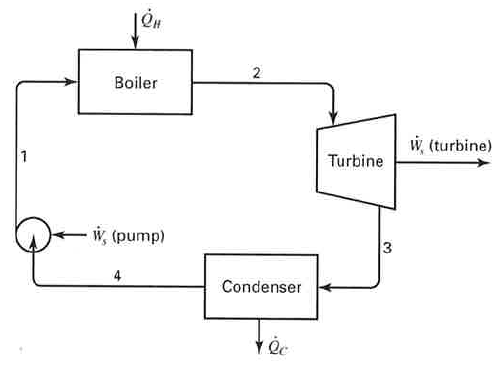
\includegraphics [width=4in]{problem_04_diagram.png}

\end{par} \vspace{1em}
\begin{par}
From the data given above, determine the following:
\end{par} \vspace{1em}
\begin{par}
a) What is the thermal efficiency for the Rankine cycle?
\end{par} \vspace{1em}
\begin{par}
The pump operates reversibly, so the work done to the system by the pump, $\dot{W}_s$, does not change the enthalpy of the steam. Therefore, $H_1=H_4$. The heat transfer from the boiler accounts for the change in enthalpy between steps 1 and 2, $\dot{Q}_H = H_2 - H_1$. Finally, because the turbine operates adiabatically, the difference in enthalpy between steps 2 and 3 is due to the shaft work done by the turbine, $\dot{W}_s = H_3 - H_2$. The efficiency of the Rankine cycle is therefore, $$ \eta = \frac{\dot{W}_s}{\dot{Q}_H} = \frac{H_3'-H_2}{H_2'-H_1} $$
\end{par} \vspace{1em}
\begin{par}
The enthalpy and entropy data for this problem are taken from a superheated steam table. The turbine exhaust quality is found by relating entropy between the turbine and condenser.
\end{par} \vspace{1em}
\begin{par}
Calculation in MATLAB:
\end{par} \vspace{1em}
\begin{verbatim}
u = symunit;
P_2 = 8000 * u.kPa;
T_2 = rewrite(400 * u.Celsius, u.K, 'Temperature', 'absolute');
T_4 = rewrite(100 * u.Celsius, u.K, 'Temperature', 'absolute');
H_2 = 3141.6 * u.kJ / u.kg;
H_4 = 419.06 * u.kJ / u.kg;
H_1 = H_4;
Q_H = H_2 - H_1;
S_3_prime = 6.3694 * u.kJ / (u.kg * u.K);
S_3_liquid = 1.3069 * u.kJ / (u.kg * u.K);
Delta_S_condensation = 6.04985 * u.kJ / (u.kg * u.K);
syms x;
x = solve(S_3_prime == S_3_liquid + x*Delta_S_condensation);
H_3_liquid = 419.06 * u.kJ / u.kg;
Delta_H_condensation = (2676 * u.kJ/u.kg) - H_4;
H_3_prime = H_3_liquid + x*Delta_H_condensation;
W_s = H_3_prime - H_2;
efficiency = abs(W_s / Q_H);
vpa(efficiency, 5)
\end{verbatim}

        \color{lightgray} \begin{verbatim} 
ans =
 
0.30631
 
\end{verbatim} \color{black}
    \begin{par}
b) What is the thermal efficiency of a practical cycle with a turbine efficiency of 0.75?
\end{par} \vspace{1em}
\begin{par}
In this case, the shaft work is reduced by a quarter. The efficiency equation is still valid, $$ \eta = \dot{W}_s/\dot{Q}_H $$
\end{par} \vspace{1em}
\begin{par}
Calculation in MATLAB:
\end{par} \vspace{1em}
\begin{verbatim}
W_s_practical = 0.75 * W_s;
eff_practical = abs(W_s_practical / Q_H);
vpa(eff_practical, 5)
\end{verbatim}

        \color{lightgray} \begin{verbatim} 
ans =
 
0.22973
 
\end{verbatim} \color{black}
    \begin{par}
c) What is the quality of the turbine exhaust for the Rankine and practical cycle?
\end{par} \vspace{1em}
\begin{par}
The exhaust quality for the Rankine cycle was found as part of solving part a:
\end{par} \vspace{1em}
\begin{verbatim}
fprintf('Turbine exhaust quality (Rankine): %.5f \n', vpa(x));
\end{verbatim}

        \color{lightgray} \begin{verbatim}Turbine exhaust quality (Rankine): 0.83680 
\end{verbatim} \color{black}
    \begin{par}
To find the exhaust quality for the practical cycle, $H_3$ is calculated in terms of the revised shaft work. This is related to the table values for enthalpy to find the exhaust quality, $$ H_3 = \dot{W}_s + H_2 = H_3^L + x\Delta{H}_{cond} $$ Calculation in MATLAB:
\end{par} \vspace{1em}
\begin{verbatim}
syms x_practical;
x_practical = solve(W_s_practical + H_2 == ...
    H_3_liquid + x_practical*Delta_H_condensation);
fprintf('Turbine exhaust quality (Practical): %.5f \n', vpa(x_practical));
\end{verbatim}

        \color{lightgray} \begin{verbatim}Turbine exhaust quality (Practical): 0.92917 
\end{verbatim} \color{black}
    

\subsection*{Problem 5}

\begin{par}
The contents of the freezer in a home refrigerator are maintained at $-20~\textup{C}$. If heat leaks amount to $120,000~\textup{kJ}$ per day, and the cost of electricity is \$ $0.08/\textup{kWh}$, estimate the yearly cost of running the refrigerator. Assume a coefficient of performance equal to 60\% of the Carnot value.
\end{par} \vspace{1em}
\begin{par}
Assuming the temperature in the house is $25~\textup{C}$, the refrigeration cycle includes the heat leak as $Q_C$. Therefore, the work done by the refrigerator is equal to the heat leak divided by the coefficient of performance of the refrigerator. The yearly cost is the price of electricity multiplied by this work.
\end{par} \vspace{1em}
\begin{par}
Calculation in MATLAB:
\end{par} \vspace{1em}
\begin{verbatim}
u = symunit;
T_C = rewrite(-20 * u.Celsius, u.K, 'Temperature', 'absolute');
T_H = rewrite(25 * u.Celsius, u.K, 'Temperature', 'absolute');
performance_carnot = T_C / (T_H - T_C);
performance = performance_carnot * 0.6;
Q_C = 120000 * u.kJ / u.d;
W = Q_C / performance;
price = 0.08 / u.kWh;
cost = rewrite(W * price, u.year_Gregorian^-1);
fprintf('Cost: $%.2f per year \n', double(separateUnits(cost)))
\end{verbatim}

        \color{lightgray} \begin{verbatim}Cost: $288.56 per year 
\end{verbatim} \color{black}
    


\end{document}
    
